Die Konstruktion wurde in 3 einzelne Teile aufgeteilt: Bodenplatte, hinterer Aufbau und Lenkung. Diese Teile sind mit wenigen Schrauben und Steckverbindung voneinander trennbar. Dies wurde gemacht, um den Transport und die Lagerung zu vereinfachen.\\
Der Aufbau wurde in Inventor geplant und konstruiert.\\
\begin{figure}[H]
    \centering
    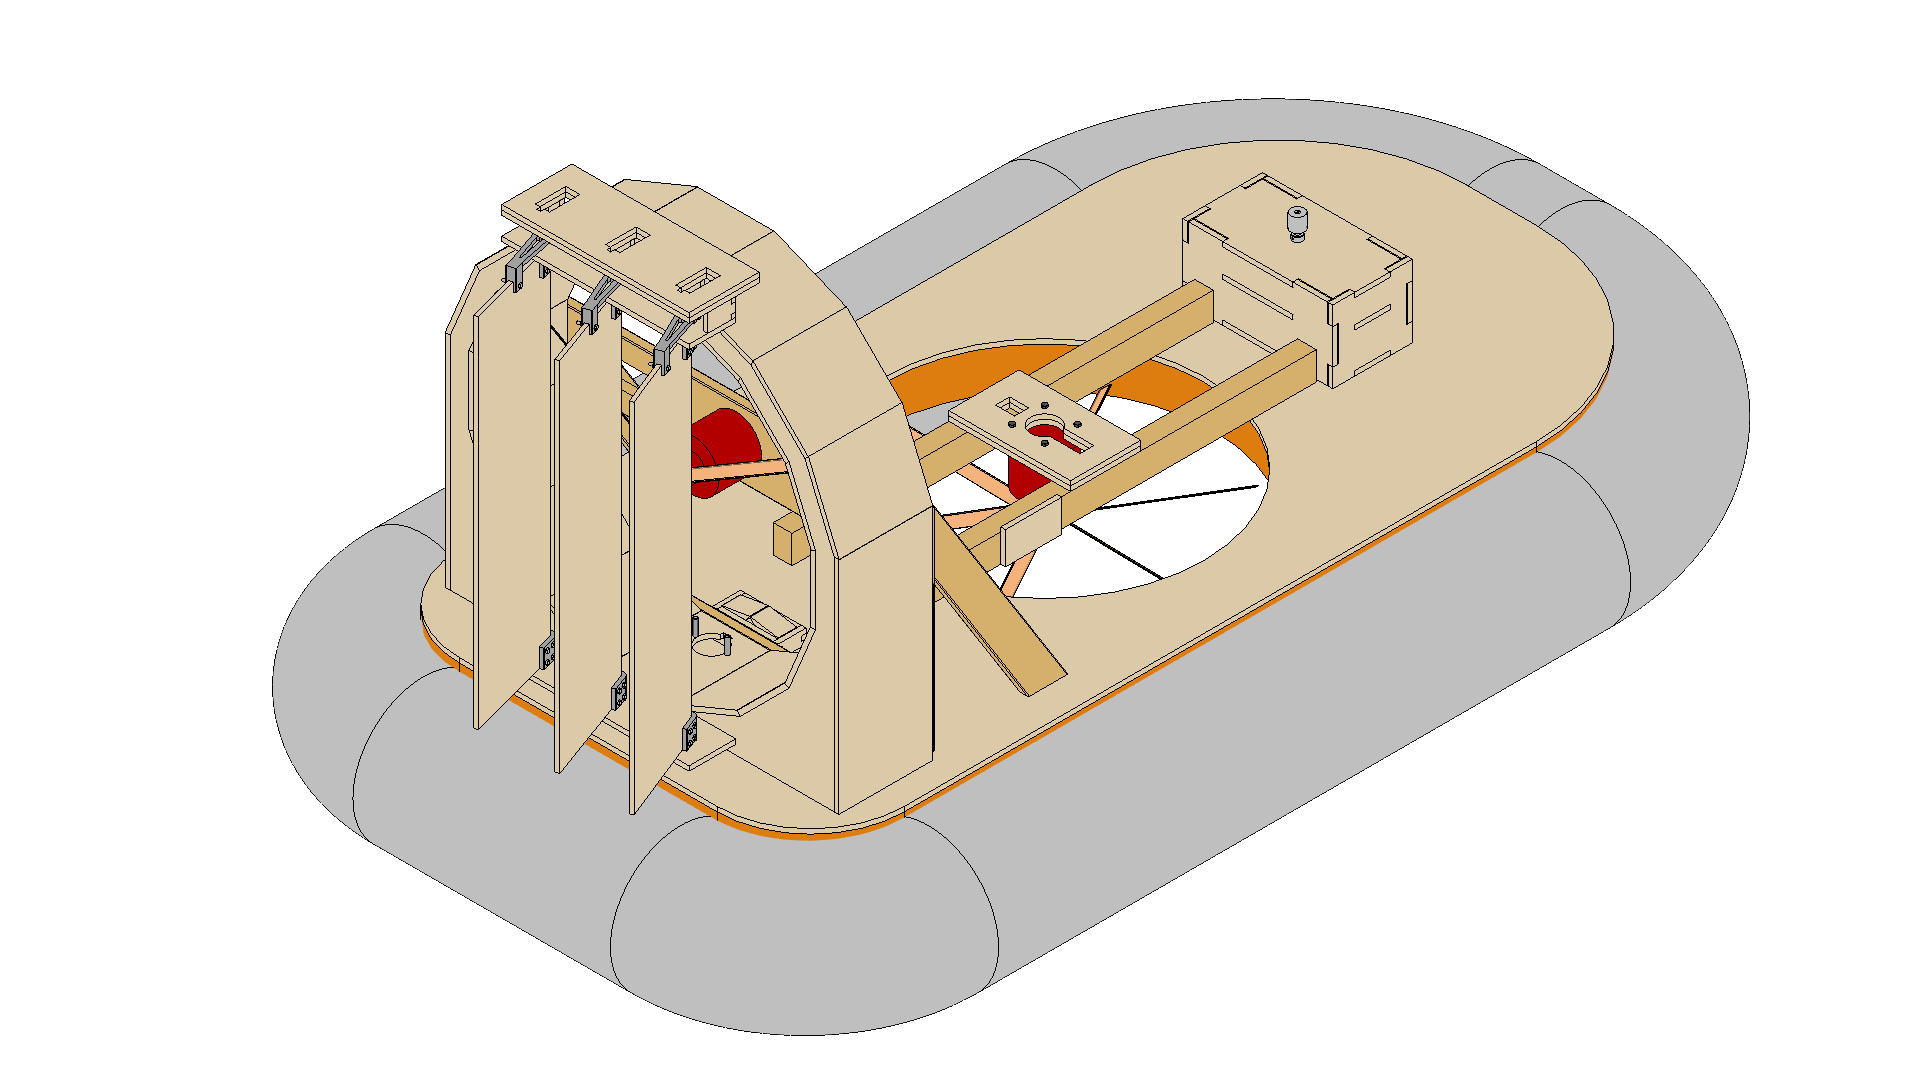
\includegraphics[width=\textwidth]{../Inventor/Luftkissenboot.png}
    \caption{Konstruktion 3D-Modell gesamt}
\end{figure}

\clearpage
\section{Bodenplatte}
Die Bodenplatte ist die Grundlage auf welcher die anderen beiden Teile befestigt sind und stellt die Verbindung mit dem Boot da.\\
Um die Bodenplatte möglichst leicht aber trotzdem stabil zu halten wurde XPS in Verbindung mit Pappelsperrholz verwendet.\\
% Die Bodenplatte wurde aus 10cm dicken XPS--Platten und einer 1cm dicken Pappelsperrholzplatte zusammengesetzt. In das XPS wurden zur Verstärkung noch links und rechts 2 20x95\,mm Holzlatten eingefräst und eingeklebt.\\ 
In der Mitte der Bodenplatte wurde das Loch für den Propeller ausgeschnitten. Im XPS wurde der Lochdurchmesser so gewählt, dass der Propeller darin frei drehen kann. Der Lochdurchmesser in der Holzplatte darüber wurde um 2\,cm kleiner gewählt um zu verhindern das am Rand des Loches die Luft direkt wieder hinausströmt.

\begin{figure}[H]
    \centering
    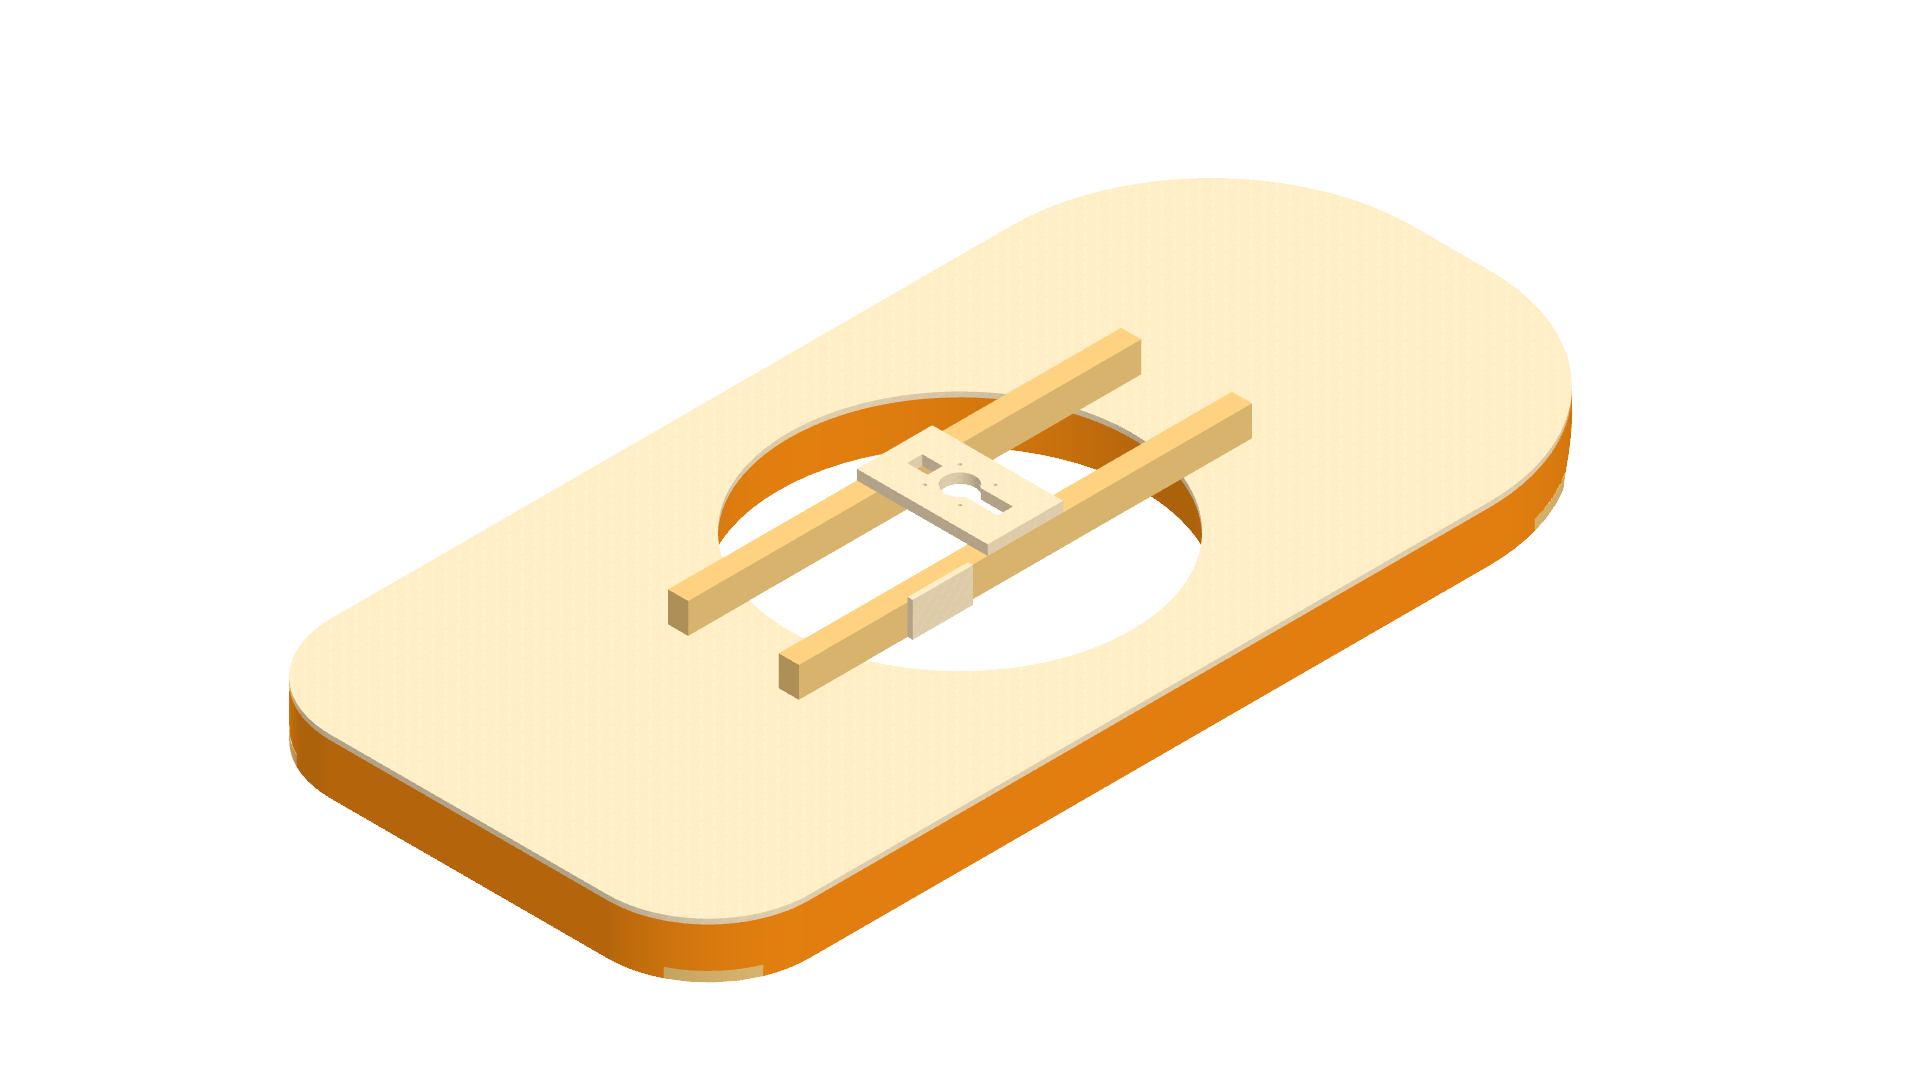
\includegraphics[width=\textwidth]{../Inventor/Bodenplatte/png/BodenplatteHauptansicht.png}
    \caption{Bodenplatte 3D-Modell\label{fig:konst:bodenplatte:gesamt}}
\end{figure}

\subsection{Stückliste}
\begin{table}[H]
    \centering
    \begin{tabular}{|c|M{4.5cm}|M{3.5cm}|c|c|}
        \hline
        \textbf{Stk} & \textbf{Name} & \textbf{Material} & \textbf{Herstellung} & \textbf{Abbildung}\\\hline
        1 & Bodenplatte Pappel  & 10mm Pappel & Stichsäge & \ref{fig:bodenplatte:skizze:BodenplattePappel}\\\hline
        1 & Bodenplatte XPS & 100mm XPS & Messer & \ref{fig:bodenplatte:skizze:BodenplatteXPS1}, \ref{fig:bodenplatte:skizze:BodenplatteXPS2}\\\hline
        1 & Verstärkung Holzlatte links & Holzlatte Fichte 20x90mm & Kappsäge & \ref{fig:bodenplatte:skizze:VHOLZL}\\\hline
        1 & Verstärkung Holzlatte rechts & Holzlatte Fichte 20x90mm & Stichsäge & \ref{fig:bodenplatte:skizze:VHOLZR}\\\hline
        2 & Staffel Motorhalterung & Staffel gehobelt 40x60mm & Stichsäge & \ref{fig:bodenplatte:skizze:Staffel}\\\hline
        2 & Platte Motorhalterung & 10mm Pappel & LaserCutter & \ref{fig:bodenplatte:skizze:Motorhalterung}\\\hline
        1 & Platte Motorregler-Halterung & 10mm Pappel & LaserCutter & \ref{fig:bodenplatte:skizze:Motorreglerhalterung}\\\hline
        1 & Gitter unten & Lochplatte & Gekauft & ??\\\hline
    \end{tabular}
    \caption{Stückliste Bodenplatte}
    \label{tab:konst:bodenplatte:stueckliste}
\end{table}
\todo{add ref}

\subsection{Inventor}
\begin{figure}[H]
    \centering
    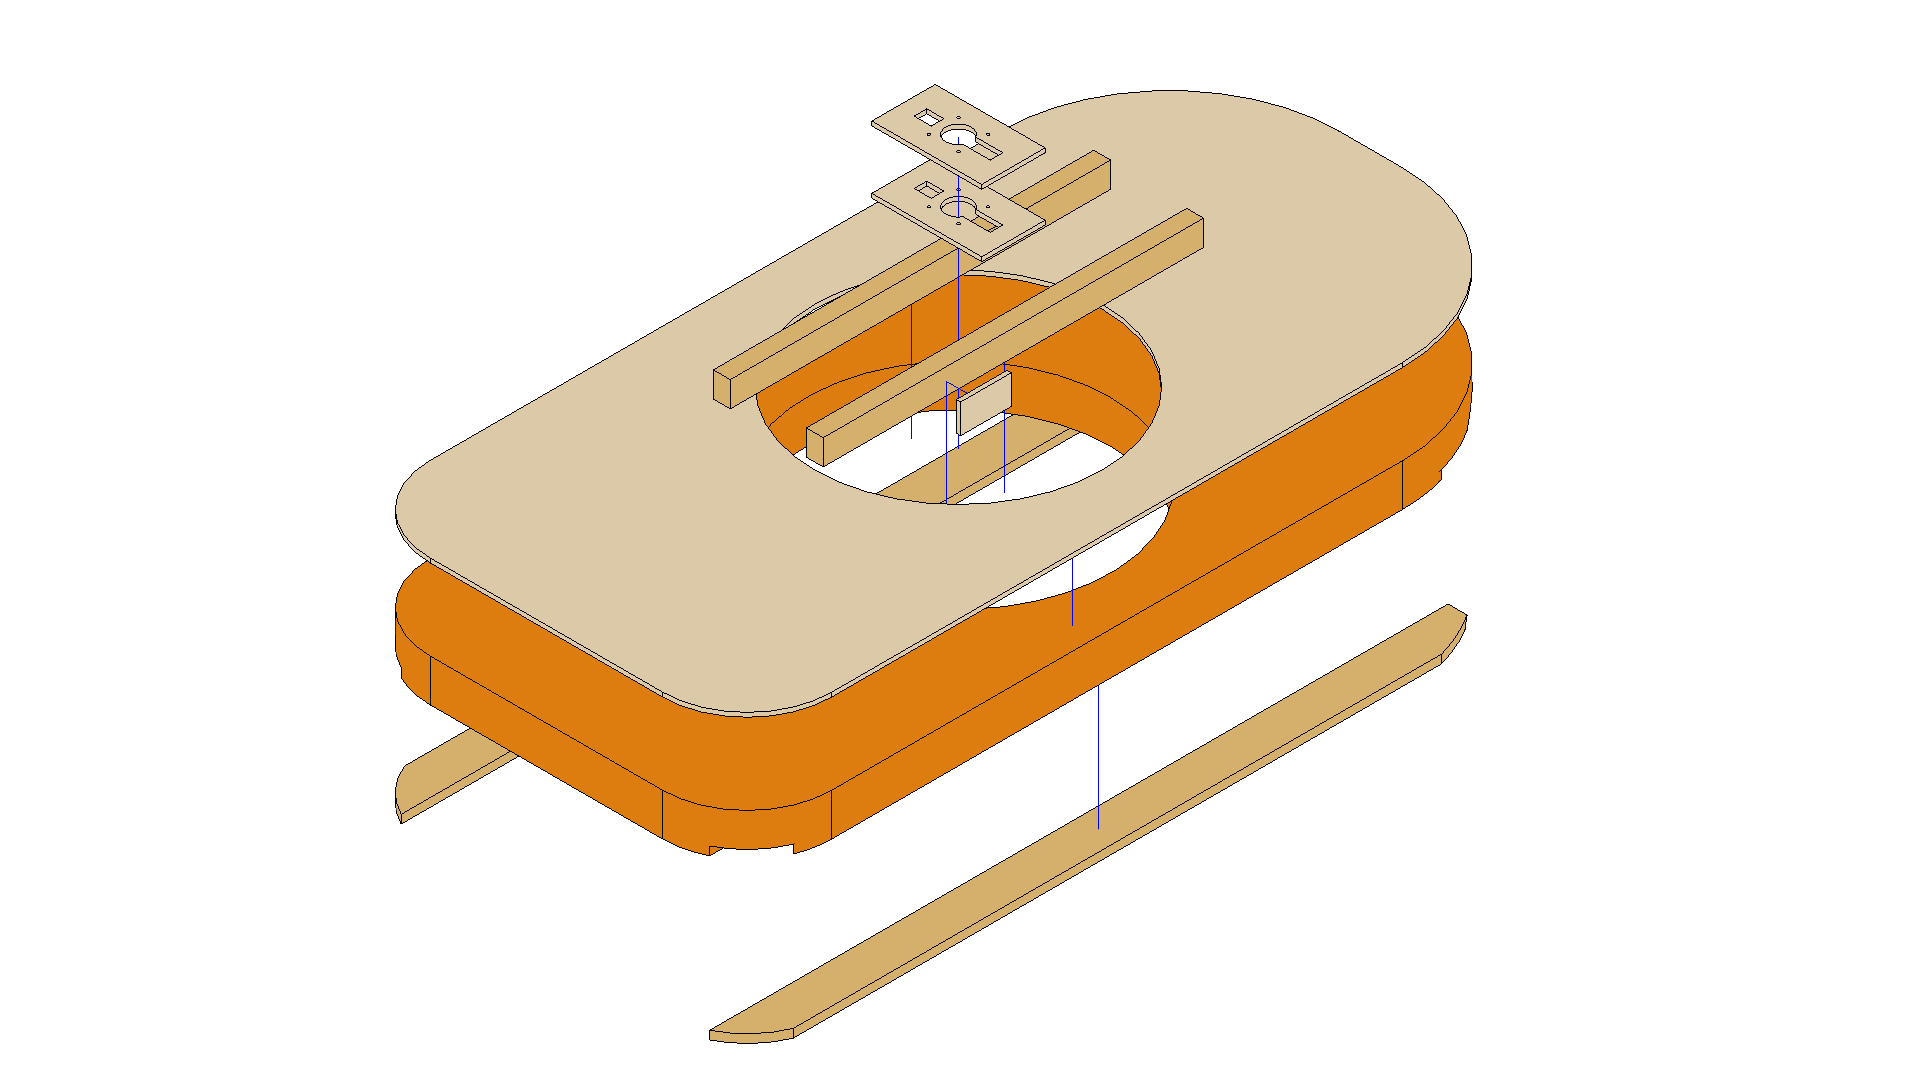
\includegraphics[width=\textwidth]{../Inventor/Bodenplatte/png/Bodenplatte_Praesentation_Hauptansicht.png}
    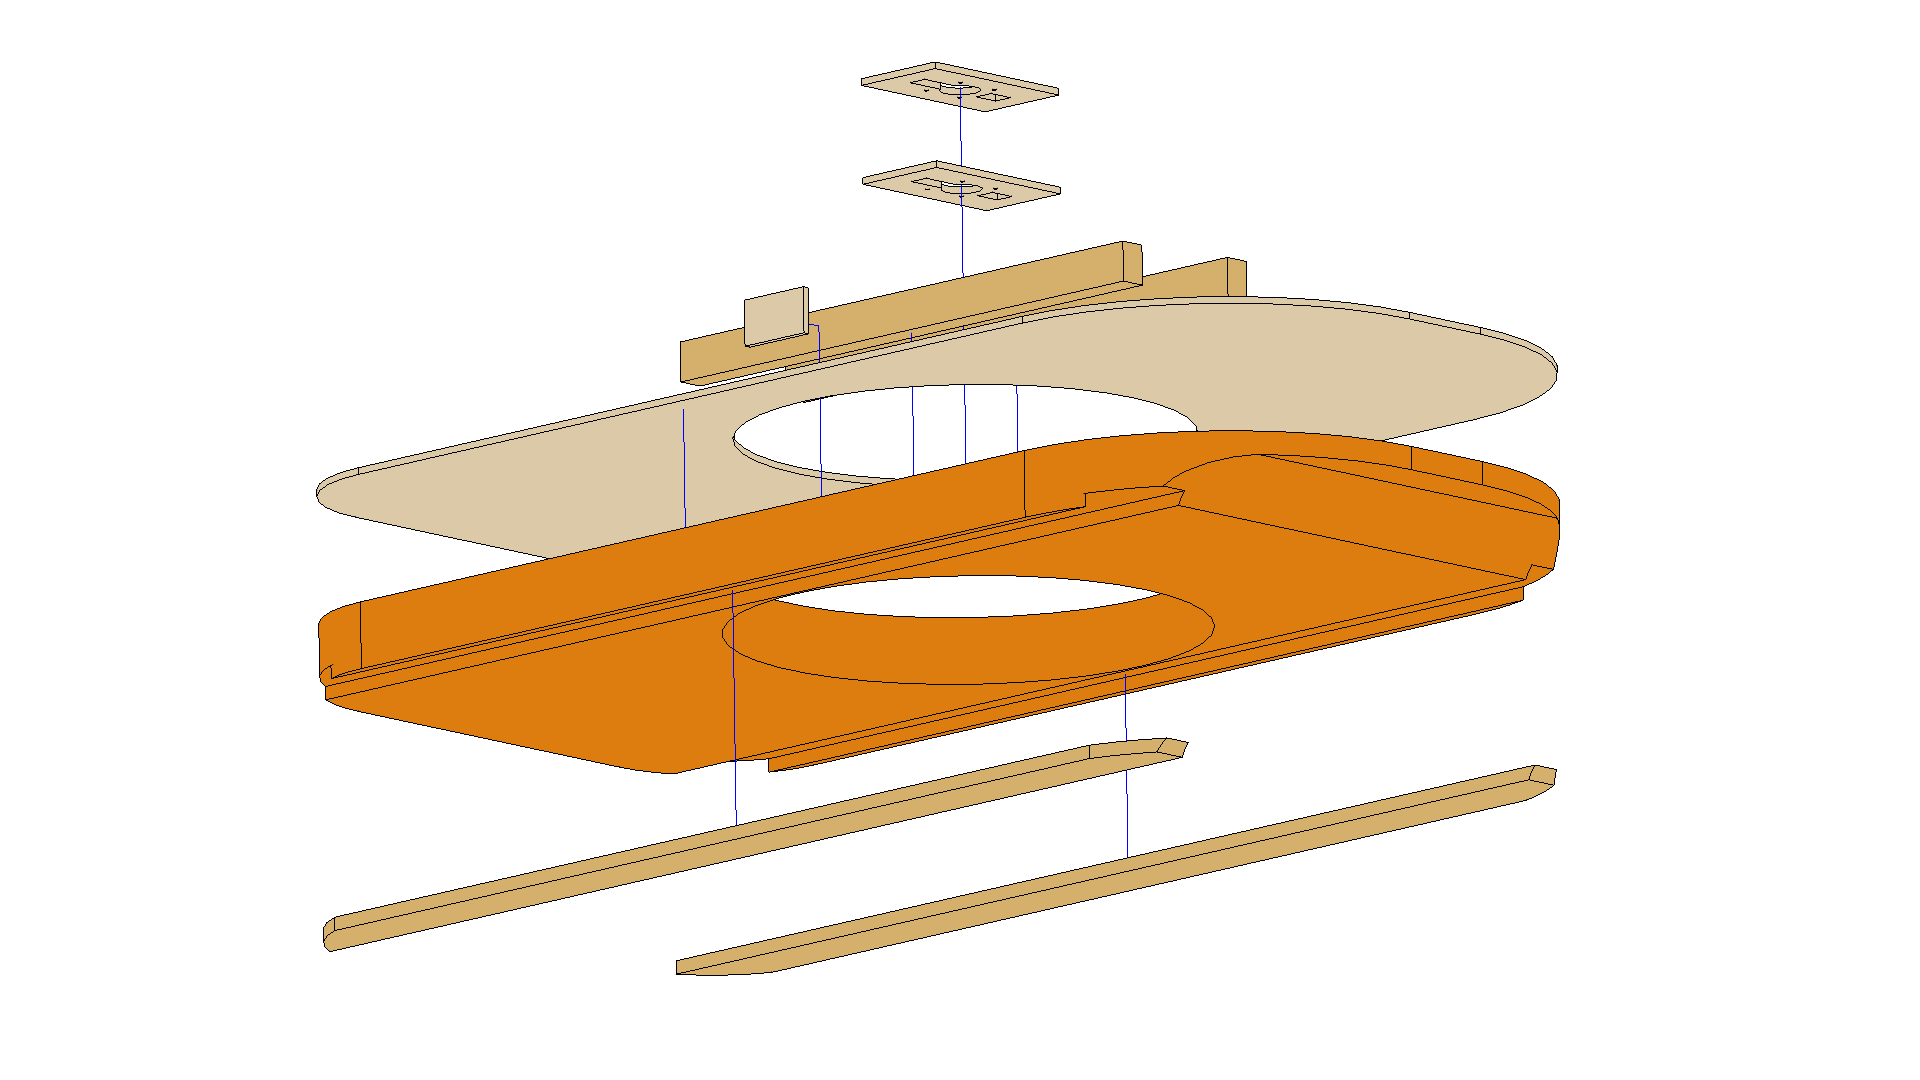
\includegraphics[width=\textwidth]{../Inventor/Bodenplatte/png/Bodenplatte_Praesentation_SeitlichUnten.png}
    \label{fig:konst:bodenplatte:inventor}
    \caption{Bodenplatte Inventor Explosionsansicht}
\end{figure}
\clearpage

\begin{landscape}
    \includeSkizze{../Inventor/Bodenplatte/Zeichnung/Bodenplatte-Holz.pdf}{Bodenplatte Pappel}{fig:bodenplatte:skizze:BodenplattePappel}{1}
    \clearpage

    \includeSkizze{../Inventor/Bodenplatte/Zeichnung/Bodenplatte-XPS.pdf}{Bodenplatte XPS 1}{fig:bodenplatte:skizze:BodenplatteXPS1}{1}
    \clearpage
    \includeSkizze{../Inventor/Bodenplatte/Zeichnung/Bodenplatte-XPS.pdf}{Bodenplatte XPS 2}{fig:bodenplatte:skizze:BodenplatteXPS2}{2}
    \clearpage

    \includeSkizze{../Inventor/Bodenplatte/Zeichnung/HolzLatteLinks.pdf}{Verstärkung Holzlatte links}{fig:bodenplatte:skizze:VHOLZL}{1}
    \clearpage

    \includeSkizze{../Inventor/Bodenplatte/Zeichnung/HolzLatteRechts.pdf}{Verstärkung Holzlatte rechts}{fig:bodenplatte:skizze:VHOLZR}{1}
    \clearpage

    \includeSkizze{../Inventor/Bodenplatte/Zeichnung/40x60Staffel.pdf}{Staffel Motorhalterung}{fig:bodenplatte:skizze:Staffel}{1}
    \clearpage

    \includeSkizze{../Inventor/Bodenplatte/Zeichnung/Motorhalterung.pdf}{Motorhalterung}{fig:bodenplatte:skizze:Motorhalterung}{1}
    \clearpage

    \includeSkizze{../Inventor/Bodenplatte/Zeichnung/HalterungMotorregler.pdf}{Motorregler-Halterung}{fig:bodenplatte:skizze:Motorreglerhalterung}{1}
    \clearpage

    \missingfigure{Foto Gitter?}
    \clearpage
\end{landscape}


\cleardoublepage
\subsection{Zusammenbau}
Die XPS-Platte wurde aus 4 einzelnen 100mm dicken XPS-Platten zusammengeklebt und mit einem Messer zugeschnitten. Die Schlitze für die Holzlatten wurden mit einer Oberflächenfräse eingefräst und die Holzlatten (\autoref{fig:bodenplatte:skizze:VHOLZL} \&\ \autoref{fig:bodenplatte:skizze:VHOLZR}) wurden mit Silikon eingeklebt.\\
Die Pappelsperrholzplatte wurde mit 8 M8x120mm Schrauben mit der XPS-Platte verschraubt.\\
Danach wurde das Metallgitter angeschraubt und die Staffel zur Motorhalterung wurden darüber geleimt und geschraubt.\\ 
\missingfigure{Fotos Bodenplatte reintuen}

\subsection{Monatage am Boot}
Die Bodenplatte soll möglichst luftdicht mit dem Schlauchboot verbunden werden. Um dies zu erreichen wurde eine Teichfolie mit doppelseitigem Klebeband am Boot angeklebt und an der Holzplatte mit einer Leiste angeschraubt.\\
Um die Unterseite des Bootes beim bremsen zu schützen, wurde ein Stück aus einer Bodenplatte ausgeschnitten und mit Pattex Kraftkleber an das Boot geklebt.\\
Um ein Verrutschen der Konstruktion verhindern, wurde die Bodenplatte zusätzlich mit Lochband am Boot befestigt -- siehe \todo{add ref fotot}
\missingfigure{add foto lochband befestigung}


\clearpage
\section{Aufbau hinten}
Der hintere Aufbau beinhaltet den Motor für den Vortrieb, sowie die Fahnen zum Lenken. Die 3 Fahnen werden von 3 Servos angesteuert.\\ Außerdem sind die Akkus und die Kupferschienen zur Stromverteilung im unteren Teil des Aufbaus versteckt. Um die Akkus erreichbar zu machen sind die zwei äußeren Platten aufklappbar.


\subsection{Stückliste}
\begin{table}[H]
    \centering
    \begin{tabular}{|c|M{4.5cm}|M{3.5cm}|c|c|}
        \hline
        \textbf{Stk} & \textbf{Name} & \textbf{Material} & \textbf{Herstellung} & \textbf{Abbildung}\\\hline
        2 & Hauptplatte & 10mm Pappel & Stichsäge & \ref{fig:Aufbau:skizze:hauptplatte}\\\hline
        1 & Platte innen unten & 10mm Pappel & Stichsäge & \ref{fig:Aufbau:skizze:innenUnten}\\\hline
        14 & Platten innen 1 schräge Kante & 10mm Pappel & Handkreissäge & \ref{fig:Aufbau:skizze:innen1seite}\\\hline
        1 & Platte innen 2 schräge Kanten & 10mm Pappel & Handkreissäge & \ref{fig:Aufbau:skizze:innen2seite}\\\hline
        1 & Platte außen oben & 10mm Pappel & Stichsäge & \ref{fig:Aufbau:skizze:assenOebn}\\\hline
        4 & Platte außen 1 schräge Kante & 10mm Pappel & Handkreissäge & \ref{fig:Aufbau:skizze:aussen1seite}\\\hline
        2 & Platte außen 2 schräge Kanten & 10mm Pappel & Handkreissäge & \ref{fig:Aufbau:skizze:assen2seite}\\\hline
        2 & Platte außen Seite & 10mm Pappel & Handkreissäge & \ref{fig:Aufbau:skizze:aussengross}\\\hline
        1 & Verstärkung hinten Mitte & 10mm Pappel & Stichsäge & \ref{fig:Aufbau:skizze:vhintenmitte}\\\hline
        2 & Verstärkung hinten Unten & 10mm Pappel & Stichsäge & \ref{fig:Aufbau:skizze:vhintenunten}\\\hline
        2 & Verstärkung hinten schräg & 10mm Pappel & Stichsäge & \ref{fig:Aufbau:skizze:vhintenschraeg}\\\hline
        1 & Verstärkung unten & 10mm Pappel & Handkreissäge & \ref{fig:Aufbau:skizze:vunten}\\\hline
        2 & Servo Halter seitlich & 10mm Pappel & LaserCutter & \ref{fig:Aufbau:skizze:shs}\\\hline
        2 & Servo Halter seitlich 2& 10mm Pappel & LaserCutter & \ref{fig:Aufbau:skizze:shs2}\\\hline
        1 & Servo Halter hinten& 10mm Pappel & LaserCutter & \ref{fig:Aufbau:skizze:shh}\\\hline
        1 & Servo Halter lang& 10mm Pappel & LaserCutter & \ref{fig:Aufbau:skizze:shl}\\\hline
        2 & Servo Halter Hauptplatte& 10mm Pappel & LaserCutter & \ref{fig:Aufbau:skizze:shhp}\\\hline
        2 & Kabelbox Platte kurz& 10mm Pappel & LaserCutter & \ref{fig:Aufbau:skizze:kbk}\\\hline
        2 & Kabelbox Platte lang& 10mm Pappel & LaserCutter & \ref{fig:Aufbau:skizze:kbl}\\\hline
        2 & Kabelbox Deckel& 10mm Pappel & LaserCutter & \ref{fig:Aufbau:skizze:kbd}\\\hline
        2 & Fahnenhalter Hauptteil& PETG & 3D-Drucker & \ref{fig:Aufbau:skizze:fhh}\\\hline
        2 & Fahnenhalter Servo& PETG & 3D-Drucker & \ref{fig:Aufbau:skizze:fhs}\\\hline
        2 & Fahnenhalter Rechteck& PETG & 3D-Drucker & \ref{fig:Aufbau:skizze:fhr}\\\hline        
    \end{tabular}
    \caption{Stückliste Aufbau hinten}
    \label{tab:konst:aufbau:stueckliste}
\end{table}
\todo{add 3D Druck Files}


\begin{landscape}
    \includeSkizze{../Inventor/hintererAufbau/Zeichnungen/Hauptplatte.pdf}{Hauptplatte}{fig:Aufbau:skizze:hauptplatte}{1}
    \clearpage
    \includeSkizze{../Inventor/hintererAufbau/Zeichnungen/InnenUnten.pdf}{Platte innnen unten}{fig:Aufbau:skizze:innenUnten}{1}
    \clearpage
    \includeSkizze{../Inventor/hintererAufbau/Zeichnungen/PlatteInnenEineSeite.pdf}{Platte innen 1 schräge Kante}{fig:Aufbau:skizze:innen1seite}{1}
    \clearpage
    \includeSkizze{../Inventor/hintererAufbau/Zeichnungen/PlatteInnenzweiSeiten.pdf}{Platte innen 2 schräge Kanten}{fig:Aufbau:skizze:innen2seite}{1}
    \clearpage
    \includeSkizze{../Inventor/hintererAufbau/Zeichnungen/aussenOben.pdf}{Platte außen oben}{fig:Aufbau:skizze:assenOebn}{1}
    \clearpage
    \includeSkizze{../Inventor/hintererAufbau/Zeichnungen/PlatteAussenEineSeite.pdf}{Platte außen 1 schräge Kante}{fig:Aufbau:skizze:aussen1seite}{1}
    \clearpage
    \includeSkizze{../Inventor/hintererAufbau/Zeichnungen/PlatteAussenZweiSeiten.pdf}{Platte außen 2 schräge Kanten}{fig:Aufbau:skizze:assen2seite}{1}
    \clearpage
    \includeSkizze{../Inventor/hintererAufbau/Zeichnungen/PlatteAussenGross.pdf}{Platte außen Seite}{fig:Aufbau:skizze:aussengross}{1}
    \clearpage
    \includeSkizze{../Inventor/hintererAufbau/Zeichnungen/VerstaerkungHintenMitte.pdf}{Verstärkung hinten mitte}{fig:Aufbau:skizze:vhintenmitte}{1}
    \clearpage
    \includeSkizze{../Inventor/hintererAufbau/Zeichnungen/VerstaerkungHintenUnten.pdf}{Verstärkung hinten unten}{fig:Aufbau:skizze:vhintenunten}{1}
    \clearpage
    \includeSkizze{../Inventor/hintererAufbau/Zeichnungen/VerstaerkungHintenSchraeg.pdf}{Verstärkung hinten schräg}{fig:Aufbau:skizze:vhintenschraeg}{1}
    \clearpage
    \includeSkizze{../Inventor/hintererAufbau/Zeichnungen/VerstaerkungUnten.pdf}{Verstärkung unten}{fig:Aufbau:skizze:vunten}{1}
    \clearpage
    \includeSkizze{../Inventor/hintererAufbau/Zeichnungen/HalterungServosHochSeitlich.pdf}{Servo Halter seitlich}{fig:Aufbau:skizze:shs}{1}
    \clearpage
    \includeSkizze{../Inventor/hintererAufbau/Zeichnungen/HalterungServoHochSeitlich2.pdf}{Servo Halter seitlich 2}{fig:Aufbau:skizze:shs2}{1}
    \clearpage
    \includeSkizze{../Inventor/hintererAufbau/Zeichnungen/HolzServoHalterHinten.pdf}{Servo Halter hinten}{fig:Aufbau:skizze:shh}{1}
    \clearpage
    \includeSkizze{../Inventor/hintererAufbau/Zeichnungen/HolzServoHalterHochLang.pdf}{Servo Halter lang}{fig:Aufbau:skizze:shl}{1}
    \clearpage
    \includeSkizze{../Inventor/hintererAufbau/Zeichnungen/HolzServoHalterMainPlatte1.pdf}{Servo Halter Hauptplatte}{fig:Aufbau:skizze:shhp}{1}
    \clearpage
    \includeSkizze{../Inventor/hintererAufbau/Zeichnungen/KabelBoxPlatteKurz.pdf}{Kabelbox Platte kurz}{fig:Aufbau:skizze:kbk}{1}
    \clearpage
    \includeSkizze{../Inventor/hintererAufbau/Zeichnungen/KabelBoxPlatteLang.pdf}{Kabelbox Platte lang}{fig:Aufbau:skizze:kbl}{1}
    \clearpage
    \includeSkizze{../Inventor/hintererAufbau/Zeichnungen/KabelBoxDeckel.pdf}{Kabelbox Deckel}{fig:Aufbau:skizze:kbd}{1}
    \clearpage

    \includeSkizze{../Inventor/hintererAufbau/Zeichnungen/Fahnen_Halter_hauptteil.pdf}{Fahnenhalter Hauptteil}{fig:Aufbau:skizze:fhh}{1}
    \clearpage
    \includeSkizze{../Inventor/hintererAufbau/Zeichnungen/Fahnen_Halter_obenTeileServo.pdf}{Fahnenhalter Servo}{fig:Aufbau:skizze:fhs}{1}
    \clearpage
    \includeSkizze{../Inventor/hintererAufbau/Zeichnungen/Fahnen_Halter_rechteck.pdf}{Fahnenhalter Rechteck}{fig:Aufbau:skizze:fhr}{1}
    \clearpage
    
   
    
\end{landscape}